
\begin{figure}[htbp]
	\centering
	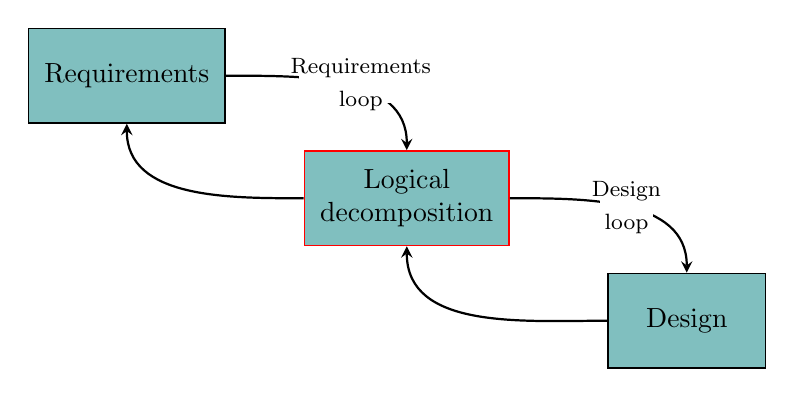
\begin{tikzpicture}
		
		\tikzstyle{function}=[rectangle,
			fill=teal!50,draw=black,semithick,
			minimum height=1.2cm,minimum width=2cm,inner sep=2mm,
			align=center,node distance=2.2cm]

		\node[function]	(reqs)	{Requirements};
		\node[function,below right of=reqs,xshift=2cm,draw=red]	(logical)	{Logical\\ decomposition};
		\node[function,below right of=logical,xshift=2cm]	(design)	{Design};

		\draw[->,>=stealth,thick,out=0,in=90] (reqs) to node[fill=white,inner sep=-1mm,xshift=2mm,align=center]{\footnotesize Requirements\\\footnotesize  loop} (logical);
		\draw[<-,>=stealth,thick,out=270,in=180] (reqs) to (logical);

		\draw[->,>=stealth,thick,out=0,in=90] (logical) to node[fill=white,inner sep=-1mm,align=center]{\footnotesize Design\\\footnotesize  loop} (design);
		\draw[<-,>=stealth,thick,out=270,in=180] (logical) to (design);

	\end{tikzpicture}
	\caption{The Logical Decomposition phase}
	\label{fig:decomposition}
\end{figure}
